\chapter{Results}\label{res:results}

The results for the analog blocks were obtained by using spectre simulator in CADENCE. In case of noise simulation a transient noise was imposed. The functionality and integrity of the modulator and the analog blocks were validated using Nominal simulation. Additionally PVT simulations were performed on the modulator,the OTAs and the quantizer in order to verify the robustness of these blocks. The nominal simulation operate with typical transistor model at room temperature and standard supply voltage. PVT simulation on the other hand operate with corner models of the the process where the range of the temperatures are between $-40^\circ$ and $105^\circ$, and 2.5 V and 5.5 V for the supply voltage. Furthermore it also consists of performing many simulations based on the statistical model of the transistors, namely 16. The corners model of the transistors provided by Microchip Technology are: slow, fast, slow-NMOS-fast-PMOS (SNFP) and fast-NMOS-slow-PMOS (FNSP). 


\section{Non-overlapping clock}
The output signals from the designed non-overlapping clock generator is shown in Fig. \ref{clock_out}. The non-overlapping time is 23.52nsec between $\phi_1$ and $\phi_2$, and $\phi_{1d}$ is delayed from $\phi_1$ with 10nec, the same apply for $\phi_{2d}$ and $\phi_2$. It should be noted that the delays are not affected by mismatch effects and process variation. 

\begin{figure}[h]
\centering
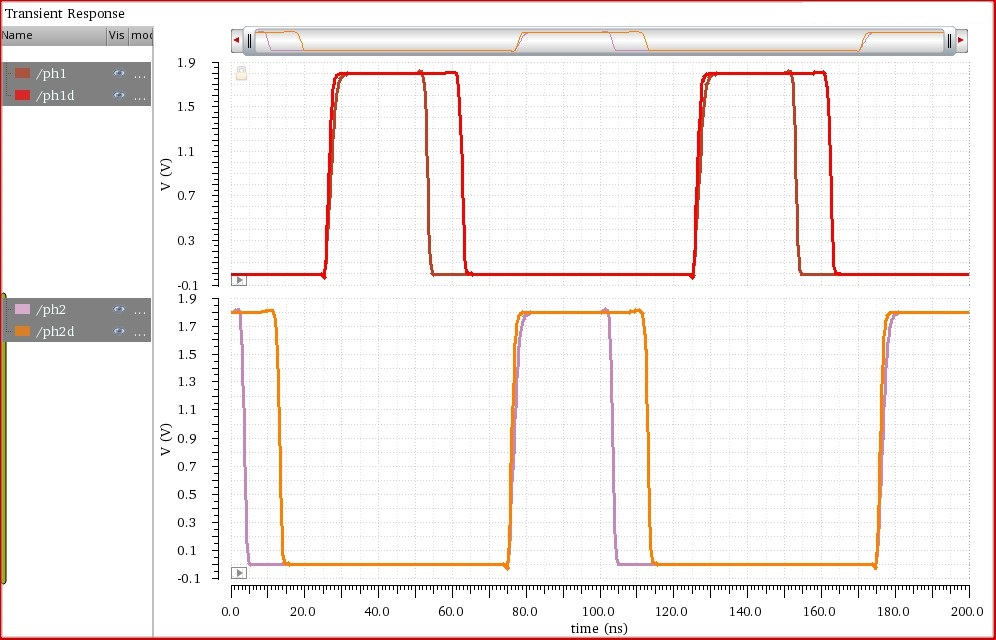
\includegraphics[width=\textwidth]{images/two_phase_clock_out.jpg}
\caption{Clock phases}
\label{clock_out}
\end{figure}

\section{Quantizer}
The quantizer used is simply a latched comparator which switches to the rail supply depending on the input signals. It is designed as per the methodology discussed earlier. The quantizer was simulated using three input signals: $V_{in+}$, $V_{in-}$ and CLK. The positive and negative input voltages are signals that vary from ground to $V_{DD}$ and from $V_{DD}$ to ground respectively. The output only changes at the rising edge of the clock. As mentioned in the methodology the hysteresis parameter was used to validate the quantizer, since the input offset and the input referred noise get attenuated by the feedback loop of the modulator. Figure \ref{comparator_out} shows when the output gets updated as the input voltages $V_{in+}$ and $V_{in-}$ vary. Due to the regenerative latch the hysteresis of the quantizer was measured as small as 586$\mu V/V$. PVT simulations were performed with no corners being critical to the quantizer's performance. 

\begin{figure}[H]
\centering
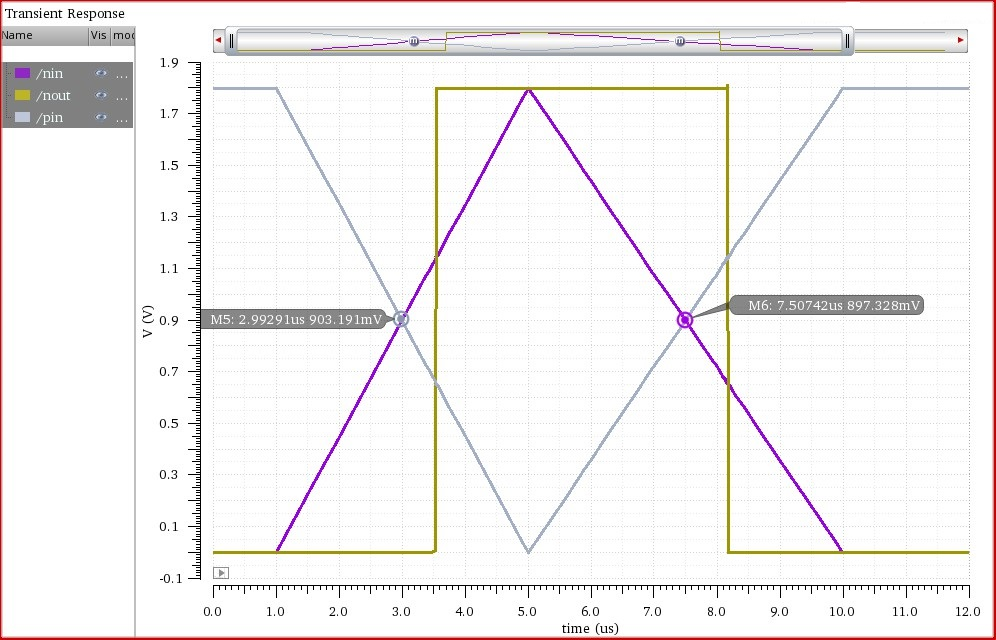
\includegraphics[width=\textwidth]{images/Comperator_output.jpg}
\caption{Hysteresis of the comparator}
\label{comparator_out}
\end{figure}


\section{OTA}
With the use of nominal and PVT simulation the specifications were validated. The results of the simulation are based on the set of requirements listed in table \ref{spec_ota}. 

\subsection{Nominal simulations}

\begin{table}[h]
\centering
\caption{Nominal results from OTA 1, 2 and 3}
\label{nominal_ota}
\begin{tabular}{l|l|l|l}
\hline
\multirow{1}{*}{Specification} & \multicolumn{1}{c|}{OTA 1} & \multicolumn{1}{c|}{OTA 2} & \multicolumn{1}{c}{OTA 3}  \\\cline{1-4}
                       
            DC gain       & 60dB & 42dB & 40dB\\
            GBW      & 43.2MHz & 36.7MHz & 38.2MHz\\
            Phase margin     & 75.6$^\circ$ & 70$^\circ$ & 78.4$^\circ$\\
            Power    & 22.3$\mu$W & 11.7$\mu$W & 8.5$\mu$W\\
            Slew rate   & 42.12MV/sec & 46.23MV/sec & 47.76MV/sec\\
            Maximum output voltage    & 1.15 & 1.2 & 1\\
            Minimum output voltage     & 0.65 & 0.65 & 0.7\\
            
\hline            
\end{tabular}
\end{table}

The main results of the nominal simulations of OTA 1, 2 and 3 are listed in table \ref{nominal_ota}, and frequency response is depicted in Fig. \ref{frequrncy_out}. AS discussed in chapter 3 the specifications of the OTAs are indeed relaxed, which made the design process that much easier. The DC-gain and GBW fulfill the specifications with good margin for all three OTAs. Even with the common mode feedback block which effect the stability, the phase margin of the three OTAs exceeds the requirements. Additionally the power consumption including the bias circuit were around 22.3 $\mu W$, 11.7$\mu W$ and 8.5$\mu W$ for OTA 1, 2 and 3 respectively. One thing to notice is that the power consumption of OTA 1 is greater than for OTA 2 and 3 due to the slew rate requirement. Different topologies can be used to reduce the power consumption of OTA 1, such as an adaptive bias circuit \cite{adaptive}. It improves the power efficiency while achieving high slew rate. 

\begin{figure}[H]
\centering
\begin{subfigure}[b]{0.85\textwidth}
   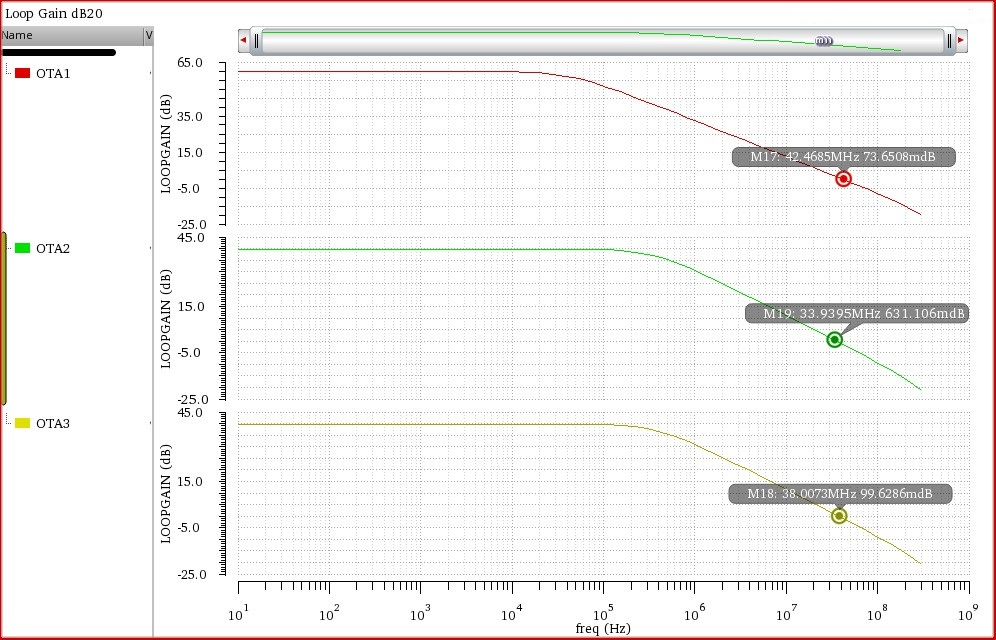
\includegraphics[width=\textwidth]{images/nom_GBW_1_2_3.jpg}
\end{subfigure}

\begin{subfigure}[b]{0.85\textwidth}
   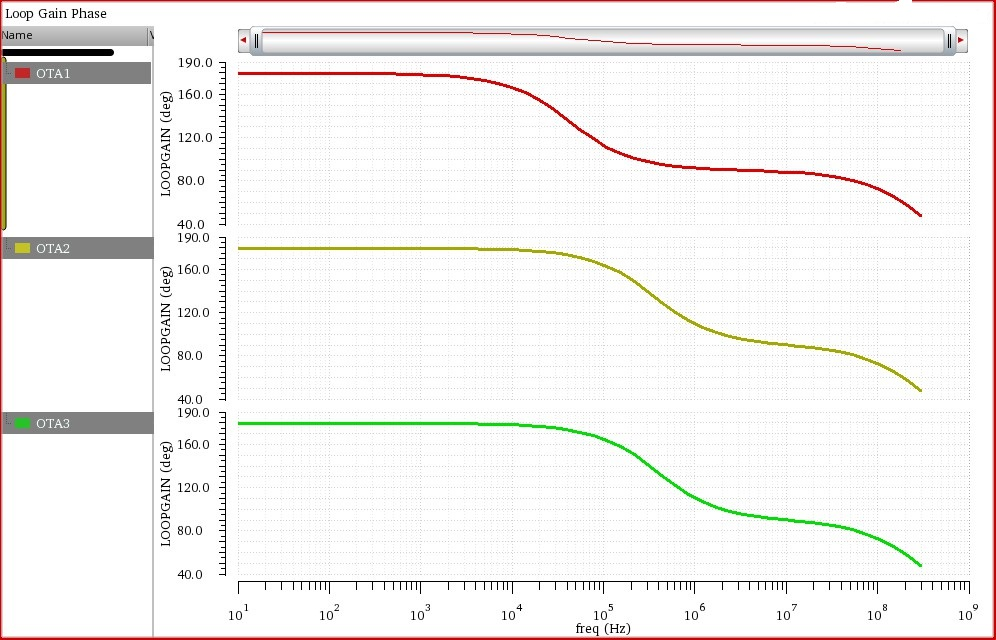
\includegraphics[width=\textwidth]{images/nom_phase_1_2_3.jpg}
\end{subfigure}

\caption{Frequency response of OTA 1,2 and 3}
\label{frequrncy_out}
\end{figure}

The maximum and minimum output voltages of OTA 1 and 2 within in the requirement in table \ref{spec_ota} with headroom to spare, since the transistors $M_3$, $M_4$, $M_9$ and $M_10$ operated in moderate region. However the maximum and minimum output voltages of OTA 3 fulfill the requirements just barley. This will not affect the performance of the modulator as it will be seen in subsequent sections. 
\begin{figure}[H]
\centering
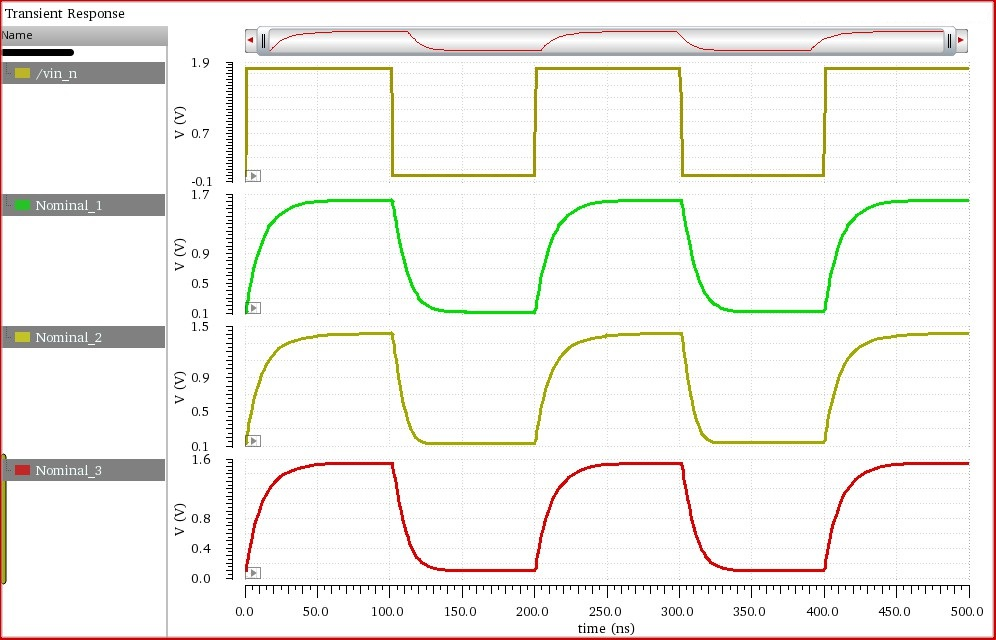
\includegraphics[width=\textwidth]{images/nominal_slew_rate_1_2_3.jpg}
\caption{Slew rate of OTA 1, 2 and 3 }
\label{slew_rate_out}
\end{figure}

The slew rates of the OTAs were found to be 42.12MV/sec, 46.23MV/sec 47.76MV/sec for OTA 1, 2 and 3 respectively, shown in Fig \ref{slew_rate_out}. With these high slew rates one can ensure that the non-linear settling error will not occur. 



\subsection{PVT simulations}
Table \ref{pvt_ota} summarize the maximum and minimum values of the OTAs 1, 2 and 3 parameters for the PVT simulations. It can be seen that the results fulfill the specifications of the amplifier. Table \ref{corners} list up the different environment used to perform the PVT simulations.


\begin{table}[H]
\centering
\caption{PVT results for OTA 1, 2 and 3}
\label{pvt_ota}
\begin{tabular}{l|l|l|l|l}
\hline
\multirow{2}{*}{Specification} & \multicolumn{2}{c|}{Minimum} & \multicolumn{2}{c}{Maximum} \\\cline{2-5}
            & Corner & Value & Corner & Value  \\\hline
            DC gain 1 &Corner 10 & 58.6dB & Corner 11 & 63.4dB \\
            DC gain 2 & Corner 6 & 39.2dB & Corner 11 & 43.3dB \\
            DC gain 3 & Corner 10 & 38.7dB & Corner 11 & 41.8dB \\\hline
            GBW 1    & Corner 3 & 40.63MHz & Corner 6 & 47.13MHz \\
            GBW 2    & Corner 3 & 33.7MHz & Corner 6 & 40.3MHz \\
            GBW 3    & Corner 3 & 34.1MHz & Corner 6 & 41.5MHz \\\hline
            Phase margin 1  & Corner 6 & 70.5$^\circ$ & Corner 13 & 81.4$^\circ$ \\
            Phase margin 2  & Corner 6 & 67.1$^\circ$ & Corner 15 & 75.5$^\circ$ \\
            Phase margin 3  & Corner 6 & 71.4$^\circ$ & Corner 15 & 82.8$^\circ$ \\\hline
            Power 1  & Corner 0 & 14.5$\mu$W & Corner 3 & 45.3$\mu$W \\
            Power 2  & Corner 0 & 7.6$\mu$W & Corner 3 & 22.5$\mu$W \\
            Power 3  & Corner 0 & 4.7$\mu$W & Corner 3 & 17.3$\mu$W \\\hline
            Slew rate 1  & Corner 5 & 36.9MV/sec & Corner 10 & 48.31MV/sec \\
            Slew rate 2  & Corner 5 & 40.3MV/sec & Corner 6 & 50.4MV/sec \\
            Slew rate 3  & Corner 5 & 38.9MV/sec & Corner 6 & 51.2MV/sec \\
            
\hline            
\end{tabular}
\end{table}

The most critical environment for all three OTAs is corner 3, where the power consumption is the largest and the GBW is the lowest. However the GBW still satisfy the requirement for the minimum allowed value for all three OTAs to assure a stable charge transfer.

\begin{table}[H]
\centering
\caption{PVT Corners}
\label{corners}
\begin{tabular}{l|l|l|l}
\hline
\multirow{1}{*}{Corners} & \multicolumn{1}{c|}{Transistor model} & \multicolumn{1}{c|}{Supply voltage} & \multicolumn{1}{c}{Temperature} \\\cline{1-4}
                       
            Corner 0       & slow & 2.5 V & -40$^\circ$\\
            Corner 1      & slow & 2.5 V & 105$^\circ$\\
            Corner 2      & slow & 5.5 V & -40$^\circ$\\
            Corner 3      & slow & 5.5V & 105$^\circ$\\
            Corner 4      & fast & 2.5 V & -40$^\circ$ V\\
            Corner 5      & fast & 2.5 V & 105$^\circ$\\
            Corner 6      & fast & 5.5 V &-40$^\circ$\\
            Corner 7      & fast & 5.5 V & 105$^\circ$\\
            Corner 8      & SNFP & 2.5 V & -40$^\circ$V\\
            Corner 9      & SNFP & 2.5 V & 105$^\circ$\\
            Corner 10      & SNFP & 5.5 V & -40$^\circ$\\
            Corner 11      & SNFP & 5.5 V & 105$^\circ$\\
            Corner 12      & FNSP & 2.5 V& -40$^\circ$\\
            Corner 13      & FNSP & 2.5 V & 105$^\circ$\\
            Corner 14      & FNSP & 5.5 V & -40$^\circ$\\
            Corner 15      & FNSP & 5.5 V & 105$^\circ$\\
            
\hline            
\end{tabular}
\end{table}

Power consumption nearly double of the nominal values for all three OTAs in corner 3, with the consumption of OTA 1 being noticeable big of 45.4 $\mu W$. The technique mentioned in the previous section can be used to reduce it.   

Figures \ref{corner_freq_1}, \ref{corner_freq_2} and \ref{corner_freq_3} illustrate the plots of the frequency responses for all corners for OTA 1, 2 and 3 respectively. As seen the DC gain for OTA 1 and 3 are worst in corner 10, while for OTA 2 it is worst in corner 6. Both corners have high supply voltage and low temperature. Nevertheless the DC gains satisfy the specifications of table \ref{spec_ota} with good margin. The phase margins also fulfill the specifications in the worst corner 6, and thereby ensuring fastest settling time.  

\begin{figure}[H]
\centering
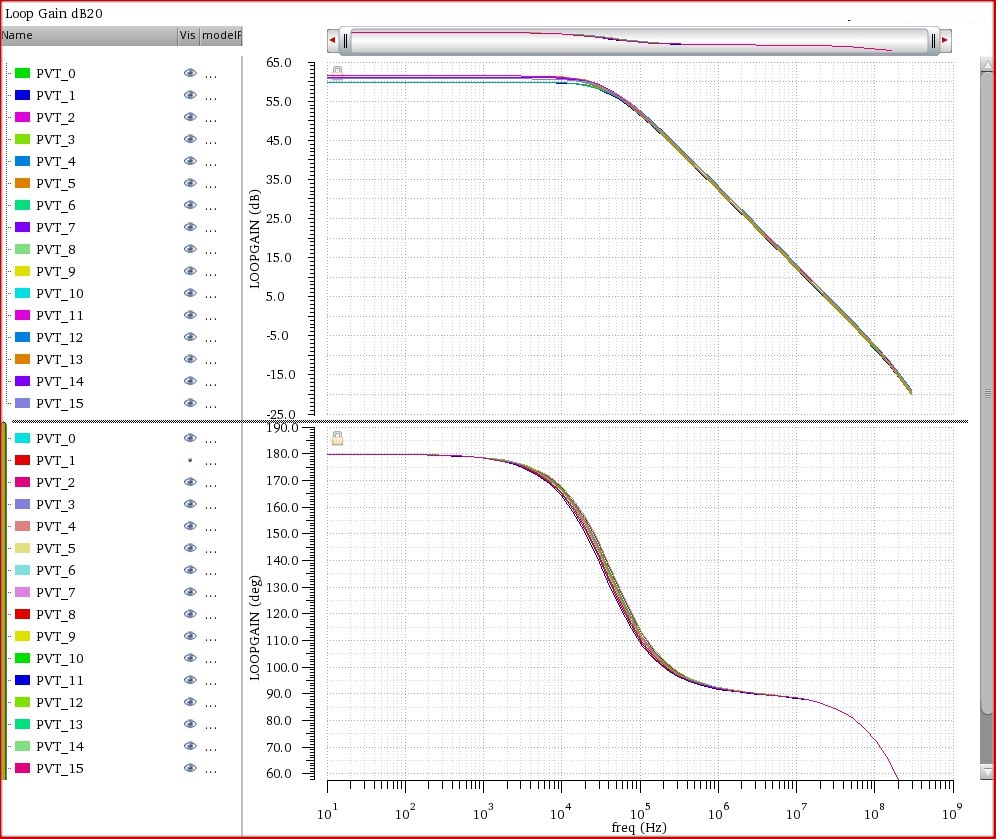
\includegraphics[width=\textwidth]{images/corner_gbw_phase_1.jpg}
\caption{Corner simulation of the OTA 1 frequency response}
\label{corner_freq_1}
\end{figure}

\begin{figure}[H]
\centering
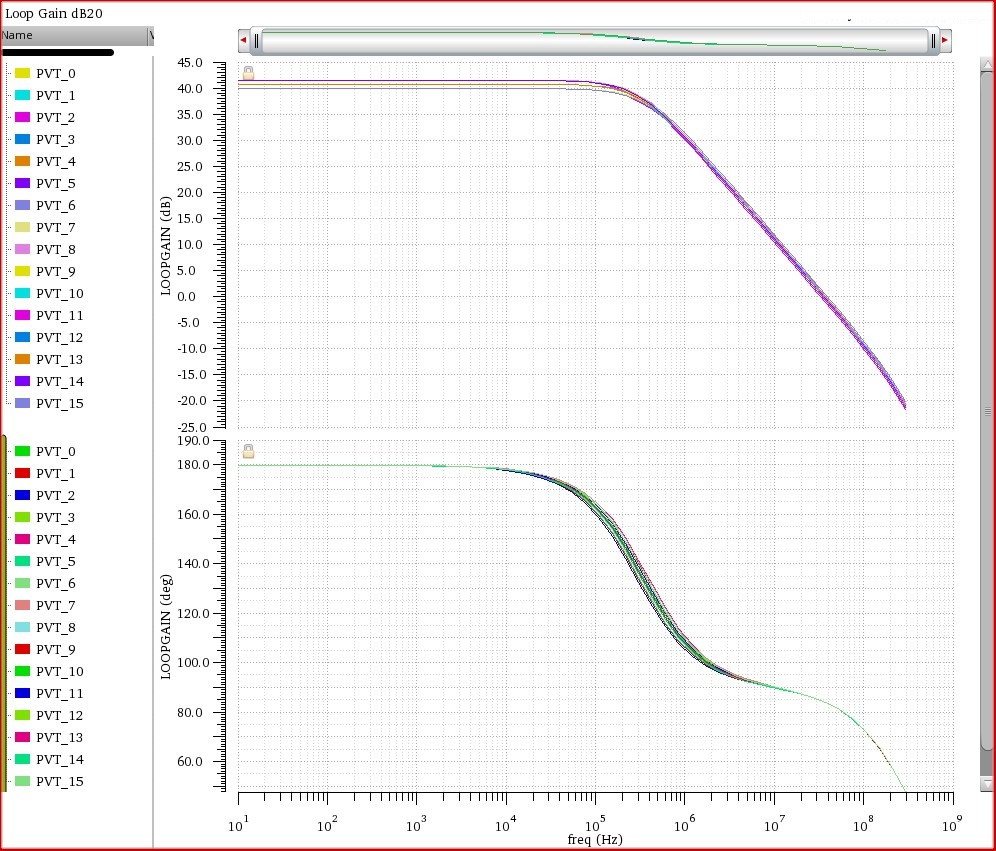
\includegraphics[width=\textwidth]{images/corner_gbw_phase_2.jpg}
\caption{Corner simulation of the OTA 2 frequency response}
\label{corner_freq_2}
\end{figure}


\begin{figure}[H]
\centering
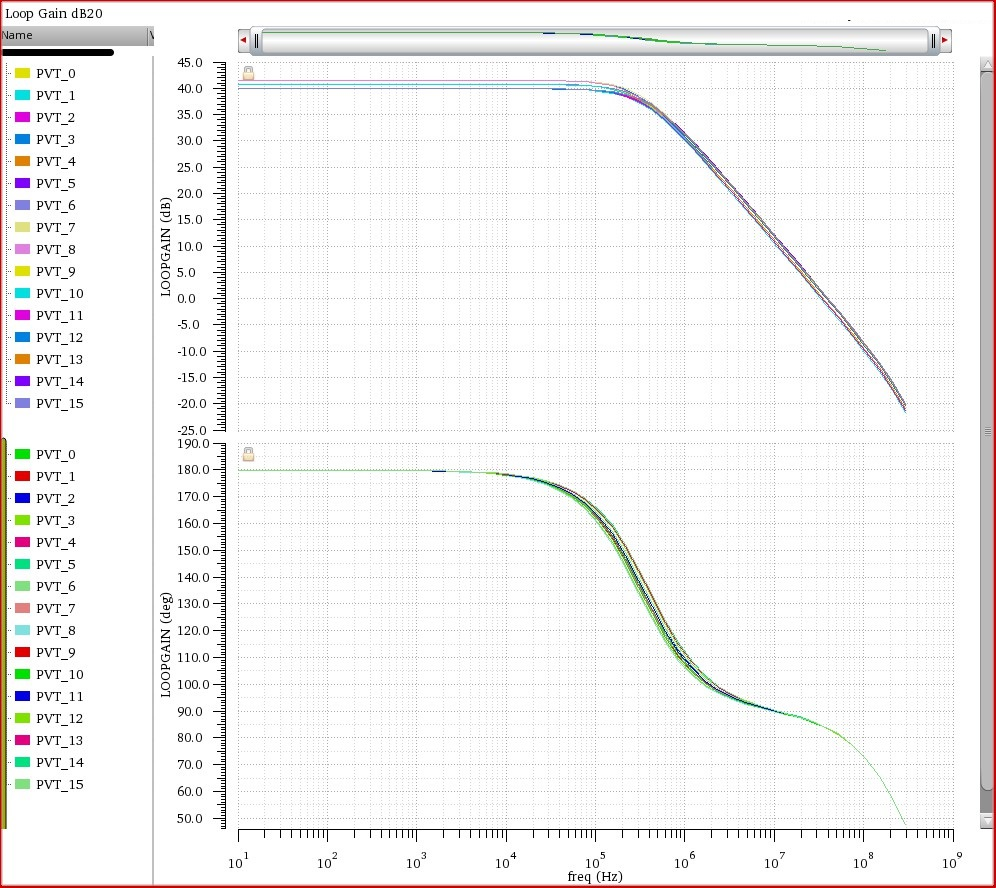
\includegraphics[width=\textwidth]{images/corner_gbw_phase_3.jpg}
\caption{Corner simulation of the OTA 3 frequency response}
\label{corner_freq_3}
\end{figure}

The slew rates for all corners for OTA 1, 2 and 3 are depicted in figures \ref{corner_slew_1}, \ref{corner_slew_2} and \ref{corner_slew_3}, and all have worst case in corner 5. With slew rates of 36.9MV/sec, 40.3MV/sec and 38.9MV/sec one can ensure a good enough settling time with good margin. 

\begin{figure}[H]
\centering
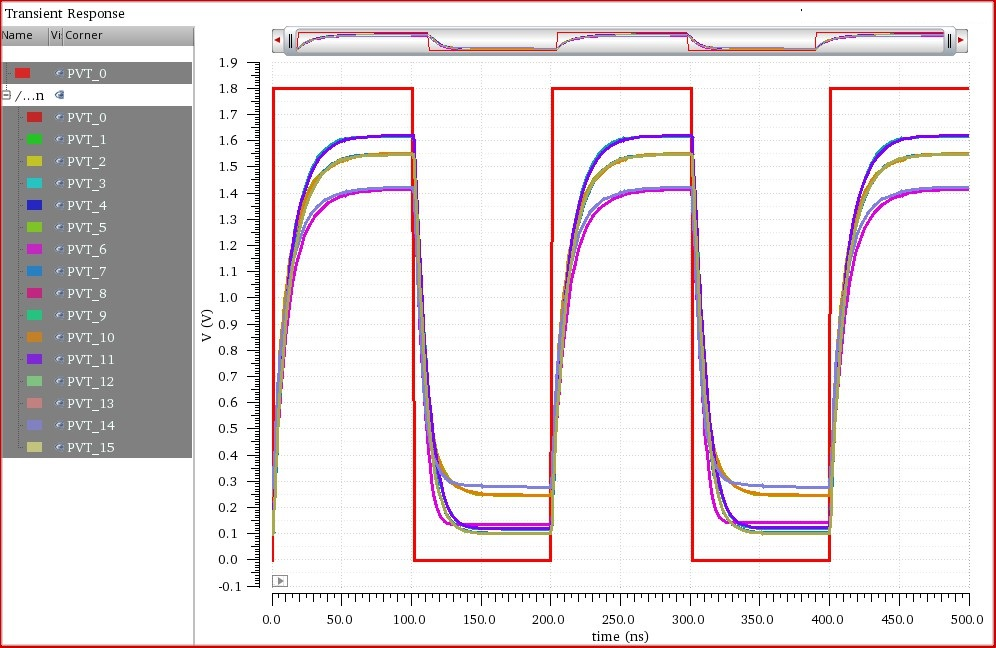
\includegraphics[width=\textwidth]{images/corner_slew_rate_1.jpg}
\caption{Corner simulation of the OTA 1 slew rate}
\label{corner_slew_1}
\end{figure}

\begin{figure}[H]
\centering
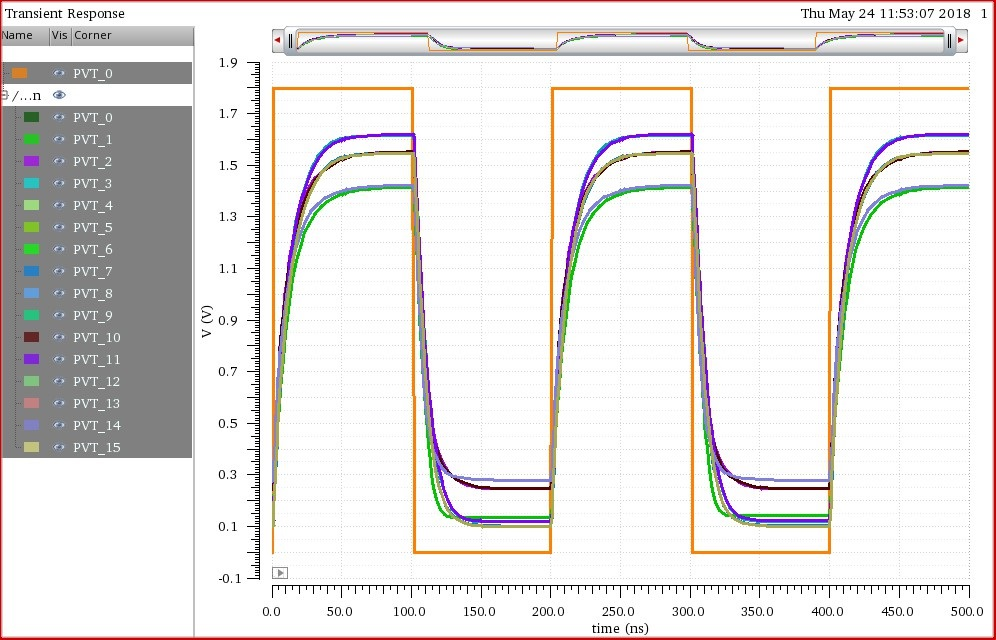
\includegraphics[width=\textwidth]{images/corner_slew_rate_2.jpg}
\caption{Corner simulation of the OTA 2 slew rate}
\label{corner_slew_2}
\end{figure}

\begin{figure}[H]
\centering
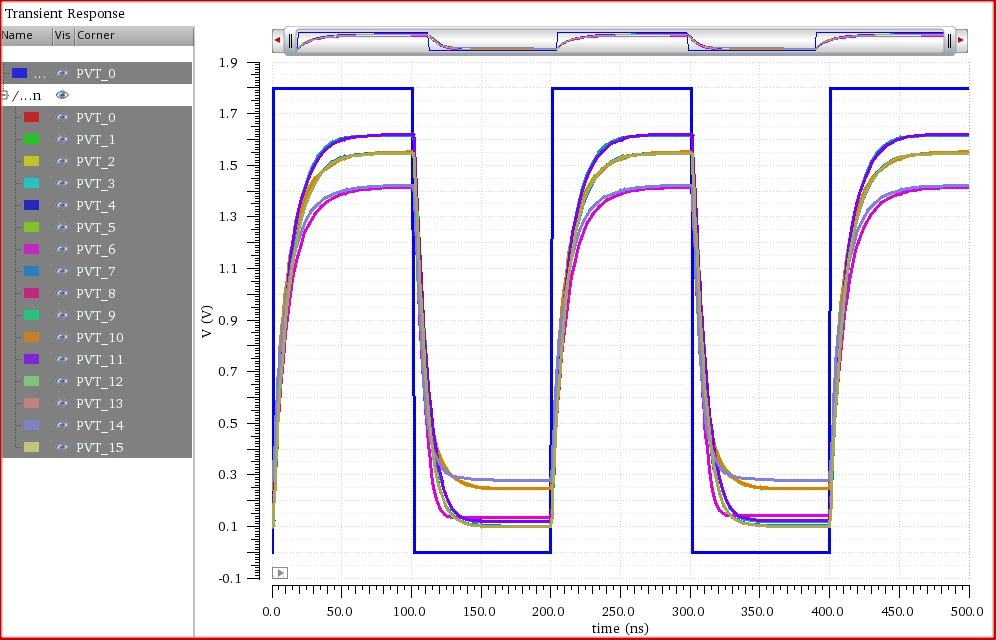
\includegraphics[width=\textwidth]{images/corner_slew_rate_3.jpg}
\caption{Corner simulation of the OTA 3 slew rate}
\label{corner_slew_3}
\end{figure}

\section{Modulator}
The response of the modulator was validated using nominal and PVT simulations with the corners listed in table \ref{corners}. A Noiseless and noisy simulations were simulated to confirm that the specification given by the thesis is achieved.  

\subsection{Noiseless simulations}
The modulator was simulates using transient analysis without imposing device noise. Nominal simulation was simulated, and the PSD of the output signal is shown in Fig \ref{psd_out}. The modulator achive a SNR of 101.20dB, a SINAD of 100.11dB and a ENOB of 16.5 bits. Here the only noise source is produced by the quantizer. 

Table \ref{modul_noiseless_out} summarize the SNRs, SINADs and ENOBs for all sixteen corners. It can be observed that all the corners fulfill the requirement of 16 bits, with corner 12 producing the lowest. Note that corner 12 is one of the corners with the lowest power consumption. 

\begin{figure}[H]
\centering
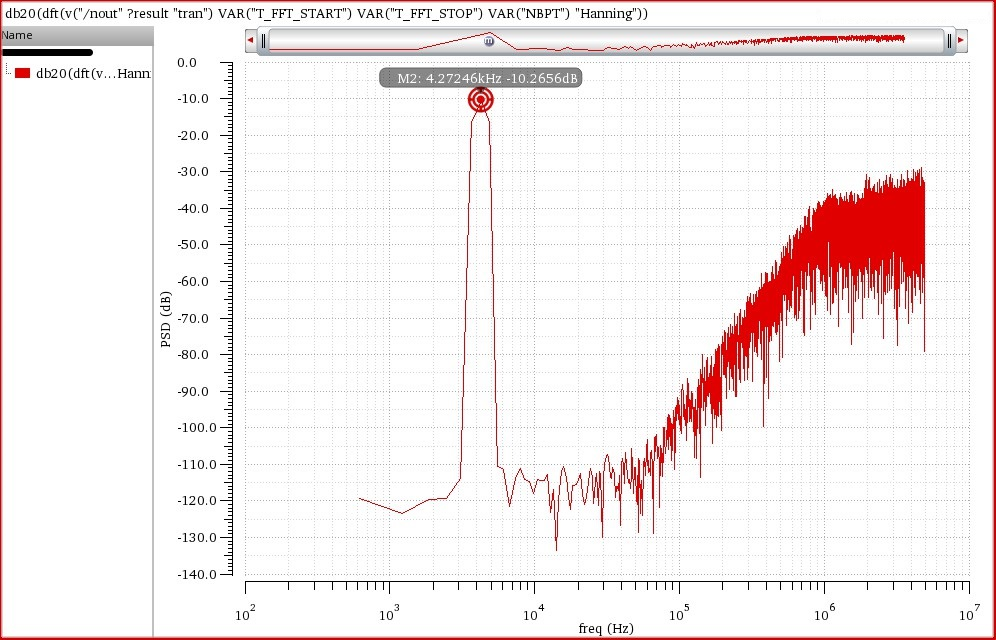
\includegraphics[width=\textwidth]{images/psd_out.jpg}
\caption{Nominal PSD of the modulator }
\label{psd_out}
\end{figure}

\begin{table}[H]
\centering

\caption{Results of the PVT simulations of the noiseless modulator}
\label{modul_noiseless_out}
\begin{tabular}{l|l|l|l}
\hline
\multirow{1}{*}{Simulation} & \multicolumn{1}{c|}{SINAD[dB]} & \multicolumn{1}{c|}{SNR[dB]} & \multicolumn{1}{c}{ENOB[bits]} \\\cline{1-4}
                       
            Nominal       &100.11 & 101.20 & 16.5\\
            Corner 0      &97.52 & 99.71 & 16.2\\
            Corner 1      &99.12 & 100.62 & 16.3\\
            Corner 2      &101.22 & 101.50 & 16.6\\
            Corner 3     &101.95 & 102.90 & 16.8\\
            Corner 4     &98.83 & 100.31 & 16.3\\
            Corner 5      &100.46 & 101.91 & 16.6\\
            Corner 6      &101.45& 101.83 & 16.6\\
            Corner 7      &100.78& 101.32 & 16.5\\
            Corner 8      &99.39& 100.84 & 16.4\\
            Corner 9      &101.94& 102.19 & 16.7\\
            Corner 10      &99.89& 101.43 & 16.6\\
            Corner 11      &101.86& 102.31 & 16.7\\
            Corner 12      &96.29& 97.30 & 16.1\\
            Corner 13      &98.54& 99.62 & 16.2\\
            Corner 14      &100.67& 101.44 & 16.5\\
            Corner 15      &100.74& 101.61 & 16.5\\
            
\hline            
\end{tabular}
\end{table}

\subsection{Noise simulation}
The modulator was simulated transient noise feature of the simulator. The PSD of the output signal is depicted in Fig \ref{psd_noise_out}. The PVT simulations are listed in table \ref{modul_noisy_out} where it can be observed that all corners except corners 0 and 12 achieve the specification of 16 bit. Nonetheless this is not a big problem as it is expected when introducing noise. Furthermore 15.7 and 15.8 bits are quite close to 16. 

\begin{figure}[H]
\centering
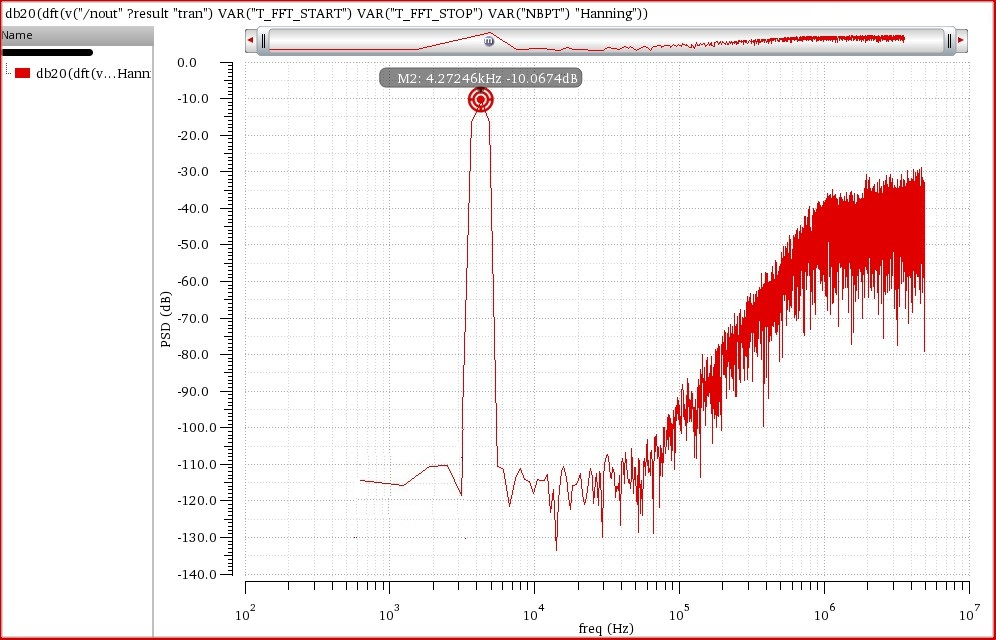
\includegraphics[width=\textwidth]{images/psd_noise_out.jpg}
\caption{Nominal noisy PSD of the modulator output }
\label{psd_noise_out}
\end{figure}

\begin{table}[H]
\centering

\caption{Results of the PVT simulations of the noisy modulator}
\label{modul_noisy_out}
\begin{tabular}{l|l|l|l}
\hline
\multirow{1}{*}{Simulation} & \multicolumn{1}{c|}{SINAD[dB]} & \multicolumn{1}{c|}{SNR[dB]} & \multicolumn{1}{c}{ENOB[bits]} \\\cline{1-3}
                       
            Nominal      &98.23 & 99.67 & 16.2\\
            Corner 0      &93.65 & 94.86 & 15.8\\
            Corner 1      &95.78 & 96.31 & 16.0\\
            Corner 2      &98.93 & 100.54 & 16.3\\
            Corner 3     &100.76 & 101.12 & 16.4\\
            Corner 4     &96.59 & 97.23 & 16.1\\
            Corner 5      &99.41 & 100.73 & 16.3\\
            Corner 6      &96.78 & 97.20 & 16.1\\
            Corner 7      &98.26 & 99.75 & 16.2\\
            Corner 8      &95.84 & 96.44 & 16.0\\
            Corner 9      &100.77 & 101.34 & 16.5\\
            Corner 10      &99.00 & 100.75 & 16.4\\
            Corner 11      &100.78 & 101.55 & 16.6\\
            Corner 12      &93.89 & 94.2 & 15.7\\
            Corner 13      &95.55 & 96.15 & 16\\
            Corner 14      &96.69 & 97.23 & 16.1\\
            Corner 15      &98.76 & 99.9 & 16.3\\
            
\hline            
\end{tabular}
\end{table}


\section{Summary of the performance }



\begin{table}[H]
\centering

\caption{Comparison with other works}
\label{comparsion_works}
\begin{tabular}{l|l|l|l|l|l}
\hline
\multirow{1}{*}{Ref.} & \multicolumn{1}{c|}{Process [$\mu$m]} & \multicolumn{1}{c|}{OSR} & \multicolumn{1}{c|}{fs [MHz]} & \multicolumn{1}{c|}{Supply [V]} & \multicolumn{1}{c}{BW [kHz]}  \\\cline{1-6}

            \cite{ref_1} & 1.5 & 64 & 10.24MHz & 5 & 160\\

\hline            
\end{tabular}
\end{table}


\begin{table}[H]
\centering

\caption{Comparison with other works continued}
\label{comparsion_works_2}
\begin{tabular}{l|l|l|l}
\hline
\multirow{1}{*}{Ref.} & \multicolumn{1}{c|}{Power [$\mu$W]} & \multicolumn{1}{c|}{SINAD [dB]} & \multicolumn{1}{c}{ENOB bit}\\\cline{1-4}

        \cite{ref_1} & 7600 & 91 & 16\\
\hline            
\end{tabular}
\end{table}